\documentclass[../main.tex]{subfiles}
\graphicspath{{../images/}}

\begin{document}

\subsection*{Lecture 1: \hfill  1/16/24}
\hrule \vspace{10px}
\section{Newtons Laws}
\hrule \vspace{10px}

\paragraph{The Four Horsemen of the Apocalypse (In Physics)}
\begin{itemize}
    \item Classical Mechanics
    \item Electromagnetism
    \item Statistical Mechanics
    \item Quantum Mechanics
\end{itemize}

Before 1900, there was no relativity or QM and the world was a simple place \dots

\paragraph{Newton's 1st Law:} The Law of Inertia

And object keeps going unless acted on by a force.

This only applies to and `inertial frame'. 

\paragraph{Newton's 2nd Law:} $\vb{F} = m\vb{a}$

Sum notation: The position vector is
\[
    \vb{r} = (x, y, z) = x(t) \vu{x} + y(t) \vu{y} + z(t) \vu{z}
\] 
in the Cartesian coordinate system. The time derivative gives the velocity
\[
    \vb{v} = \dot{\vb{r}} = \dv{\vb{r}}{t}
\]
and acceleration is the time derivative of velocity
\begin{align*}
    \vb{a} = \dot{\vb{v}} = \ddot{\vb{r}} = \dv[2]{\vb{r}}{t}
\end{align*}
Thus in vector notation, Newton's 2nd law is
\begin{align*}
    m\ddot{\vb{r}} = \vb{F}(\vb{r}, \dot{\vb{r}}, t)
\end{align*}
where $\vb{r}(t)$ is and ordinary differential equation (ODE).

The basic idea of solving mechanics problems is writing down the ODEs and solving them.

\paragraph{What is mass?} $m$ is an `inertial mass'.

In Newton's law of gravity
\begin{align*}
    \vb{F} = -\frac{GMm}{r^2} \vu{r}
\end{align*}
$m$ is the `gravitational mass' and $g \approx \qty{9.8}{\frac{m}{s^2}}$.

A larger mass has a larger inertia or `resistance to being accelerated' (Taylor). Key fact:
When acceleration is zero ($\vb{a} = 0$), the velocity is constant  ($\vb{v} = \text{constant}$).

\paragraph{Momentum:} $\vb{p} = m\vb{v}$

The third law of motion in terms of momentum is
\begin{align*}
    \vb{F} = \dot{\vb{p}} = m\dot{\vb{v}}
\end{align*}

\paragraph{Newton's Third Law:} $\vb{F}_{12} = -\vb{F}_{21}$

In a two body system, the total force of the system is
\begin{align*}
    \vb{F}_t = \vb{F}_{12} + \vb{F}_{21} = 0
\end{align*}
From the second law,
\begin{align*}
    \dot{\vb{p}}_1 = \vb{F}_{21} \qquad \dot{\vb{p}}_2 = \vb{F}_{12}
\end{align*}
adding these two equations gives
\begin{align*}
    \dot{\vb{p}}_1 + \dot{\vb{p}}_2 = 0
\end{align*}
thus the total momentum of the system is conserved.

For a system of $N$ particles, the total momentum is
\begin{align*}
    \dd{t} \sum_i \vb{p}_i = \dv{\vb{p}_{tot}}{t} = \vb{F}_{ext}
\end{align*}
sometimes $\vb{p}_{tot} = \vb{P}$ where the capital $P$ denotes the total momentum of the system.

\newpage
\subsection*{Lecture 2: \hfill  1/18/24}
\hrule \vspace{10px}
\section{A pendulum}
\hrule \vspace{10px}

\paragraph{How to solve a problem:}
\begin{enumerate}
    \item Write down the eq
    \item Solve it
    \item Understand the solution
\end{enumerate}

% figure of pendulum.png
\begin{figure*}[ht]
    \centering
    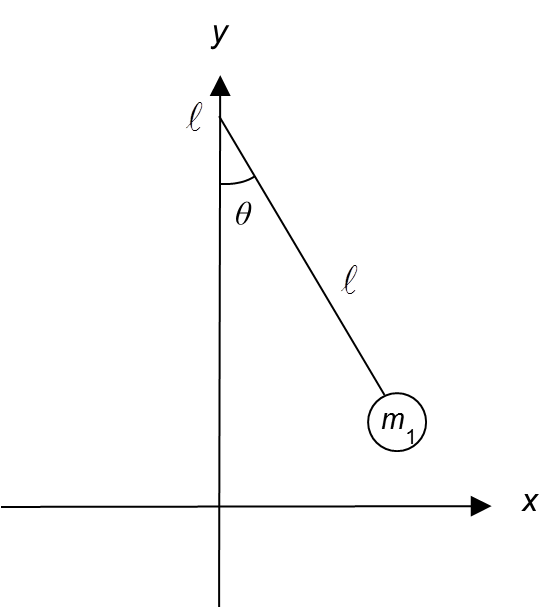
\includegraphics[width=0.4\linewidth]{pendulum.png}
    \caption{A pendulum with mass $m$ and length $l$.}
    \label{fig:2.1}
\end{figure*}    
From Figure \ref{fig:2.1}, we can write down Newton's 2nd law:
\begin{align*}
    \vb{F} &= m\vb{a} = m \ddot{\vb{r}} \\
    F_x &= -mg \sin \theta = m \ddot x \\
    F_y &= -mg \cos \theta + T \cos\theta = m \ddot x
\end{align*}
Using a right triangle we can find the angle using $\tan\theta = x/y$. Furthermore, we can use the
constrain that the length of the pendulum is constant thus $x^2 + y^2 = l^2$. But solving this
system of equations is difficult. Instead we now use a new coordinate system.

\paragraph{Quick Hack} Using the arc length $l = L\theta$ and choosing a coordinate in the direction
of the pendulums path, we can write the force equation as
\begin{align*}
    F_l = -mg \sin\theta = m \ddot l = m L \ddot \theta
\end{align*}
Thus the equation of motion is
\begin{align*}
    \ddot \theta = -\frac{g}{L} \sin\theta
\end{align*}
which is a second order ODE. This can only be solved with two conditions. We can use the initial
conditions (at $t = 0$) of the position $\theta(t = 0) = \theta_0$ and velocity $\dot\theta(0) = 0$.

\paragraph{Polar Coordinates} From Taylor:

\begin{align*}
    x &= r \cos\phi \\
    y &= r \sin\phi
\end{align*}
For an arbitrary vector $\vb{v}$ it has the Cartesian vector components
\begin{align*}
    \vb{v} = v_x \vu{x} + v_y \vu{y}
\end{align*}
Where the magnitude of the unit vectors are equivalent:
\begin{align*}
    \abs{\vu{x}} = \abs{\vu{y}} = 1
\end{align*}
and the magnitude of the vector is
\begin{align*}
    \abs{\vb{v}} &= \sqrt{\vb{v} \cdot \vb{v}} \\
    &= \sqrt{v_x^2 \vu{x} \cdot \vu{x} + 2 v_x v_y \vu{x} \cdot \vu{y} v_y^2 \vu{y} \cdot \vu{y}}\\
    &= \sqrt{v_x^2 + v_y^2}
\end{align*}
The vector $\vb{v}$ can be written in polar coordinates as
\begin{align*}
    \vb{v} = v_r \vu{r} + v_\phi \vu{\phi}
\end{align*}
where radial vector is
\begin{align*}
    \vb{r} = r \vu{r}, \qquad \vu{r} = x \vu{x} + y \vu{y}
\end{align*}
taking the time derivative of $\vb{r}$ gives the velocity
\begin{align*}
    \dot{\vb{r}} = \dot{r} \vu{r} + r \dot{\vu{r}} 
\end{align*}
but how do we find $\dot{\vu{r}}$? We can look at the change in the direction of the radial unit
vector for a small change in time $\Delta t$. Thus,
\begin{align*}
    \Delta \vu{r} \approx r \Delta\phi \vu*{\phi}
\end{align*}
dividing both sides by $\Delta t$ gives
\begin{align*}
    \frac{\Delta \vu{r}}{\Delta t} \approx r \frac{\Delta \phi}{\Delta t} \vu*{\phi}
    = r \dot\phi \vu*{\phi}
\end{align*}
Therefore, the vector in polar coordinates is
\begin{align*}
    \dot{\vb{r}} = \dot{r} \vu{r} + r \dot\phi \vu*{\phi} = v_r \vu{r} + v_\phi \vu*{\phi}
\end{align*}
where the polar components $v_r$ and $v_\phi$ are related to the radial and angular velocity
respectively. Taking the time derivative of $\dot{\vb{r}}$ gives the acceleration
\begin{align*}
    \ddot{\vb{r}} &= \ddot r \vu{r} + \dot r \dot{\vu{r}} + \dot r \dot\phi \vu{\phi} + 
    r \ddot\phi \vu{\phi} + r \dot\phi \dot{\vu\phi} \\
    &= \dot{v}_r \vu{r} + v_r \dot{\vu{r}} + \dot{v}_\phi \vu*{\phi} + v_\phi \dot{\vu*{\phi}}
\end{align*}

\newpage
\subsection*{Lecture 3: \hfill  1/22/24}
\hrule \vspace{10px}
\section{Polar Coordinates}
\hrule \vspace{10px}

using the geometric relation $\dot{\vu*{\phi}} = -\dot\phi \vu{r}$, we can write the acceleration as
\begin{align*}
    \ddot{\vb{r}} &= (\ddot r - r \dot\phi^2) \vu{r} + (r \ddot\phi + 2r \ddot\phi) \vu*{\phi} \\
    &= a_r \vu{r} + a_\phi \vu*{\phi}
\end{align*}
where $r\dot\phi^2 = r\omega^2$ is the centripetal acceleration and $r\ddot\phi = r \dot \omega$ is
the tangential acceleration.

From the Pendulum problem we know that the string is taut $r = L$ thus the radial velocity is zero
$\dot r = 0$. Thus the force equation in the $\vu*{\phi}$ direction is
\begin{align*}
    F_\phi &= m L \ddot\phi = -mg \sin\theta \\
    \ddot\phi &= -\frac{g}{L} \sin\theta
\end{align*}
which is the same equation of motion. 

\paragraph{Projectile in 2D} The initial conditions of a general projectile is usually
\begin{align*}
    F_x &= 0 = m\ddot x \\
    F_y &= -mg = m\ddot y
\end{align*}
thus the equations of motion are
\begin{align*}
    \ddot x &= 0 \\
    \ddot y &= -g
\end{align*}
And solving these equations gives the position of the projectile
\begin{align*}
    x(t) &= v_{ox} t \\
    y(t) &= y_o v_{oy} t - \frac{1}{2} g t^2
\end{align*}

This can be expanded on with the addition of air resistance $\vb{f}$. This drag force is
proportional to the velocity:
\begin{align*}
    \vb{f} \propto -\vu{v}
\end{align*}
and there are two types of air resistance: linear
\begin{align*}
    \vb{f}_l = -bv \vu{v} = -b \vb{v}
\end{align*}
and quadratic
\begin{align*}
    \vb{f}_q = -cv^2 \vu{v}
\end{align*}
where we compare the terms with
\begin{align*}
    \frac{f_l}{f_q} = \frac{cv}{b}
\end{align*}

\paragraph{Linear} $\vb{f}_l = -b \vb{v}$

From Newton's 2nd law
\begin{align*}
    F_x &= -bv_x = m\ddot x = m \dot v_x \\
    F_y &= -mg - bv_y = m\ddot y = m \dot v_y
\end{align*}
For the case of uncoupled differential equations (such as pure horizontal motion), we can solve the
horizontal equation
\begin{align*}
    \dot v_x = -\frac{b}{m} v_x 
\end{align*}
which has a general solution
\begin{align*}
    v_x = A e^{-kt}
\end{align*}
where
\begin{align*}
    k = \frac{b}{m}, \quad A = v_{ox}
\end{align*}
to find the position we have to integrate $\dot x = v_x$:
\begin{align*}
    x &= x_o + \int_0^t v_x(t') \dd{t'} \\
    &= x_o + \qt[-\frac{v_{xo}}{k} e^{-kt}]\eval_0^t
\end{align*}
where we have a limit of $t \rightarrow \infty$

For pure vertical motion, we solve the equation
\begin{align}
    \dot v_y = -g - \frac{b}{m} v_y
\end{align}
and with the initial condition $\dot v_y = 0$ we can solve for the velocity
\begin{align*}
    v_y = -\frac{mg}{b} = v_{ter}
\end{align*}
where $v_{ter}$ is the terminal velocity. To get position, we use a trick by rewriting the equation
as
\begin{align*}
    m\dot v_y = -mg - bv_y = -mg - b(v_y - v_{ter})
\end{align*}
and we can solve similar to the horizontal case using the general solution
\begin{align*}
    v_y - v_{ter} = A e^{-kt} = (v_{oy} - v_{ter}) e^{-kt}bye 
\end{align*}

\newpage
\subsection*{Lecture 4: \hfill  1/24/24}
\hrule \vspace{10px}
\section{Air Resistance}
\hrule \vspace{10px}

\paragraph{Last time:}
\begin{align*}
    \vb{f}_l &= -b \vb{v} \quad \dot{\vb{r}} = \vb{v} \\
    \vb{f}_q &= -cv^2 \vu{v}
\end{align*}
In the case of linear, $x$ motino has a range, $y$ velocity has a terminal velocity $v_t$.

\paragraph{Horizontal Quadratic Drag}
\begin{align*}
    F_y &= -mg - c\abs{v_y} v_y \\
    m\ddot y &= F_y \\
    m\dot v_y &= -mg - c\abs{v_y} v_y
\end{align*}
when $v_y = 0$ we have the terminal velocity
\begin{align*}
    v_{ter} = \sqrt{\frac{mg}{c}} \qor c = \frac{mg}{v_{ter}^2}
\end{align*}
thus the equation of motion is
\begin{align*}
    \dot v_y = -g - \frac{c}{m} v_y^2 = -g(1 - \frac{v_y^2}{v_{ter}^2}) = \dv{v_y}{t}
\end{align*}
using separation of variables
\begin{align*}
    \frac{1}{1 - \frac{v_y^2}{v_t^2}} \dd{v_y} = -g \dd{t}
\end{align*}
integrating both sides
\begin{align*}
    \int_{v_{oy}}^{v_y} \frac{1}{1 - \frac{v_y^2}{v_t^2}} \dd{v_y} = -g \int_0^t \dd{t}
\end{align*}
where we get the integral using the hyperbolic tangent
\begin{align*}
    v_t \arctanh{\frac{v_y}{v_t}} &= -gt \\
    v_y &= -v_t \tanh(gt)
\end{align*}

\paragraph{2D Motion} For Quadratic
\begin{align*}
    F_x &= -c v v_x = -c \sqrt{v_x^2 + v_y^2} v_x  = m\dot v_x \\
    F_y &= -mg - c v v_y = -mg - c \sqrt{v_x^2 + v_y^2} v_y = m \dot v_y
\end{align*}
where $v = \sqrt{v_x^2 + v_y^2}$. For linear, it is simply
\begin{align*}
    F_x &= -bv_x = m\dot v_x \\
    F_y &= -mg - bv_y = m\dot v_y
\end{align*}

\end{document}